The AI-enhanced web-based MMSE application is a sophisticated system that facilitates cognitive assessments in a digital healthcare setting\footnote{A supplementary video demonstrating the application's functionality can be accessed at \url{https://youtu.be/qnlVdwrt8n8}. This video provides a visual aid to support the technical descriptions presented in this thesis.}. This architecture seamlessly integrates modern web technologies, advanced AI capabilities, and robust security measures to provide a comprehensive and user-friendly platform for clinicians and patients. The system employs key design principles to ensure scalability, performance, and security while facilitating the integration of advanced AI capabilities for cognitive assessment.

The initial structure of the application was bootstrapped using JHipster, which provided a solid foundation with pre-configured best practices for security, testing, and API development. However, this chapter will primarily focus on the MMSE aspects of the tool, and detailed discussions on the usage of frameworks like JHipster are beyond the scope of this thesis.

\subsection{Architecture Diagram}
The AI-Powered web-based MMSE Application is built on a robust and scalable architecture, comprising several key components that work in concert to deliver efficient cognitive assessments. The system architecture consists of core components including the frontend, backend, data storage, specialized services, and external services. These components and their interactions are illustrated in a high-level architecture diagram, which can be found in Appendix \ref{appendix:system-architecture} (Figure \ref{fig:high-level-architecture}).

The system architecture consists of the following core components:
\begin{itemize}
\item \textbf{Frontend (Vue.js Application):} Delivers a responsive and intuitive user interface for clinicians and patients.
\item \textbf{Backend (Spring Boot App):} Handles core business logic, data processing, and integrations.
\item \textbf{Data Storage:} Employs PostgreSQL for persistent data storage and Redis for caching.
\item \textbf{Specialized Services:} Encompasses modules for text analysis, audio processing, NLP services, and a robust security layer.
\item \textbf{External Services:} Integrates with ChatGPT 4o API, Ollama running the Llama 3.1:70B, and MinIO for advanced functionalities.
\end{itemize}

The frontend, developed using Vue.js, delivers a responsive and user-centric interface, designed to facilitate seamless interaction for both clinicians and patients. It communicates with the backend through RESTful APIs, using JSON Web Tokens (JWT) for secure authentication and authorization \cite{Jones2015}. This approach ensures a seamless user experience while maintaining robust security measures.

\subsection{AI Integration}
Integrating AI capabilities into the MMSE application follows a hybrid model, balancing external AI services with locally deployed models. This strategy is driven by considerations of performance, data privacy, and the specialized nature of cognitive evaluations in healthcare settings \cite{Bauer2012}.

\subsubsection{AI Models and Roles}
The system integrates multiple AI models for various tasks:
\begin{enumerate}
\item \textbf{Llama 3.1:70B:} This locally deployed model, executed on the Ollama platform, is specifically optimized for complex language comprehension tasks within cognitive assessments \cite{Ollama2024}. As the primary AI engine for most MMSE tasks, Llama 3.1:70B balances high performance with robust data privacy. Utilizing local models for processing sensitive healthcare data is in accordance with best practices for safeguarding patient confidentiality in digital health applications \cite{Krutz2017}.
\item \textbf{ChatGPT 4o:} This model is employed for tasks requiring advanced language understanding and vision processing, particularly in analyzing patient-drawn figures during MMSE tasks. By interpreting these visual elements, ChatGPT 4o assists in detecting subtle cognitive impairments that might not be captured through textual responses alone. The model's ability to seamlessly integrate visual and linguistic data ensures a more comprehensive assessment, addressing the nuances of cognitive decline that are critical in early diagnosis and intervention.
\item \textbf{Transcription Model:} It converts audio inputs to text, facilitating the analysis of spoken responses. Speech analysis has been demonstrated to be a valuable tool in the early detection of cognitive impairments \cite{Konig2015}.
\item \textbf{Prediction and Similarity Models:} Employ machine learning algorithms to evaluate responses and detect subtle cognitive changes. These models are based on recent research showing the efficacy of AI in identifying early markers of cognitive decline \cite{Grassi2019}.
\end{enumerate}

Figure \ref{fig:detailed-assessment-process} provides a detailed sequence diagram of the assessment process, highlighting the data flow and decision-making steps involved in the AI-enhanced cognitive assessment.

\subsubsection{Integration Process}
\begin{figure}[h!]
\begin{center}
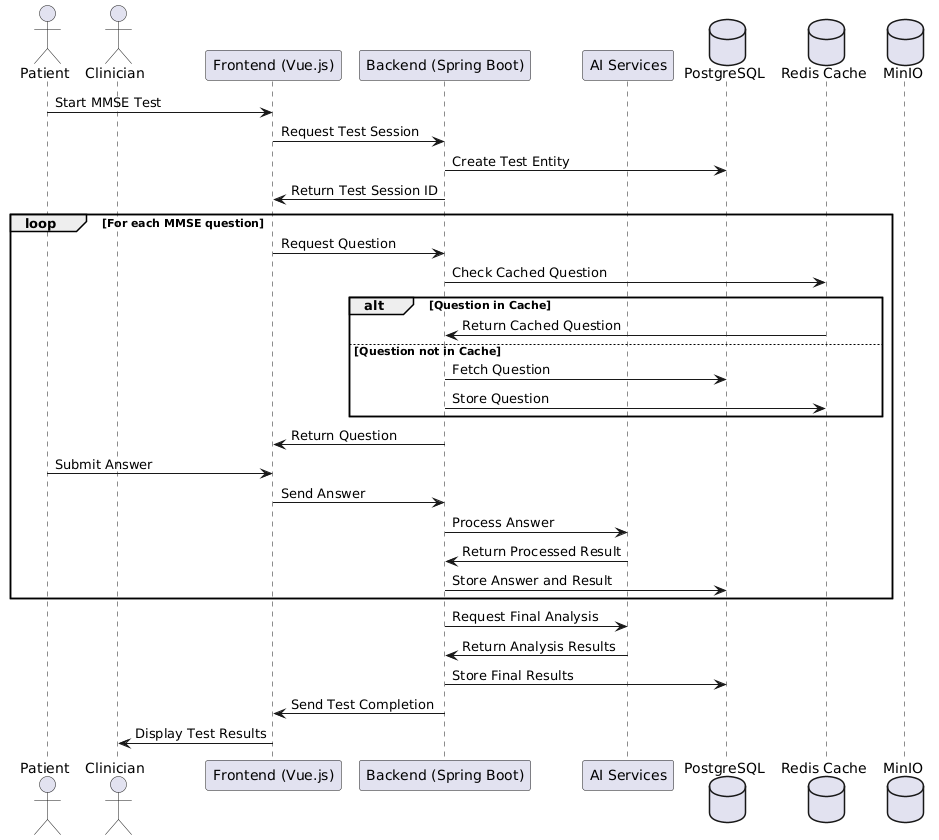
\includegraphics[width=1\textwidth]{detailed-assessment-process.png}
\caption{Detailed Assessment Process UML Diagram}
\label{fig:detailed-assessment-process}
\end{center}
\end{figure}

The AI integration process follows these key steps:
\begin{enumerate}
\item Input Processing: User input (text, audio, or images) is pre-processed and normalized.
\item Task Routing: The system routes the task to the appropriate AI model based on the input type and the question context.
\item AI Processing: The selected model processes the input and generates a response.
\item Result integration: The AI-generated results are integrated into the main application flow for scoring and analysis.
\item Fallback mechanisms: In cases where the primary AI model fails to provide a satisfactory response, the system is relegated to alternative models or human review.
\end{enumerate}

This multi-step process makes sure that the cognitive test is strong and accurate. It gets around problems with the traditional MMSE, like differences in how the test is graded and the inability to pick up on small changes in cognitive function \cite{Tombaugh1992}.

\subsubsection{Advantages of the Hybrid Approach}
The hybrid approach presents multiple advantages within the cognitive assessment domain:
\begin{itemize}
\item \textbf{Privacy Protection:} Deploying Llama 3.1:70B in a localized environment ensures that sensitive patient data is processed within a controlled and secure application framework, addressing key concerns in the security of healthcare data \cite{Krutz2017}.
\item \textbf{Enhanced Accuracy:} Combining different types of models makes cognitive tests more accurate and takes into account the person's situation. This could help find cognitive decline earlier \cite{Grassi2019}.
\item \textbf{Scalability:} The modular AI integration allows easy incorporation of new models or services as they become available, ensuring the system can adapt to advances in cognitive science and AI technology \cite{Zygouris2017}.
\item \textbf{Resilience:} Redundancy mechanisms ensure the system can handle a wide range of inputs and edge cases, crucial to maintaining reliability in clinical settings \cite{Bauer2012}.
\end{itemize}

\subsubsection{Future Extensibility}
The AI integration framework is constructed with extensibility in mind, enabling the seamless integration of emerging technologies as they evolve within the cognitive assessment field. This positions the MMSE application to evolve alongside advances in AI and cognitive science, maintaining its relevance and effectiveness in the rapidly changing field of digital healthcare. Additionally, using Ollama has made it very easy to swap models and perform integration testing to understand how many tests are failing, thereby enhancing the robustness and adaptability of the system \cite{Ollama2024, Zygouris2017}.

\subsection{Design Principles}
The Web-based MMSE application with AI is built around some key design principles that consider the difficulties of cognitive testing in a digital healthcare setting. These principles guide the overall framework and validate particular implementation decisions.

\subsubsection{Microservices and Python Services}
The decision to implement specialized services, such as text analysis and audio processing, as separate Python-based microservices using Flask stems from the need for modularity and technological flexibility. This approach allows for using specialized libraries and frameworks best suited for each task without constraining the entire system to a single technology stack. For example, the text analysis service leverages natural language processing libraries for semantic analysis, while the audio processing service utilizes specific speech recognition tools.

This microservice architecture enhances the system's scalability and maintainability. Each service can be developed, updated, and scaled independently, allowing for more efficient resource allocation and easier integration of new cognitive assessment techniques as they emerge. Moreover, this separation of concerns facilitates more robust testing and fault isolation, which are critical in a healthcare application where reliability is paramount.

\subsubsection{Architectural Design of RESTful APIs}
Implementing the RESTful API design for communication between services and the interaction between frontend and backend is based on the principles of statelessness and a uniform interface. This approach guarantees that every request from the frontend to the backend includes all the necessary information to understand and handle the request, ensuring server-side logic and enhancing scalability.

The adoption of a RESTful methodology simplifies the incorporation of external services and future system upgrades. By conforming to standard HTTP methods and status codes, the system sustains a uniform and user-friendly interface for developers, lowering the learning barrier for new team members and making documentation easier.

\subsection{Backend Implementation}
The backend of the AI-enhanced Web-based MMSE application is designed to manage business logic, data processing, and integration with external services. This section provides an overview of the backend architecture, highlighting its key components and technologies for building a robust and scalable system.

\subsubsection{Overall Structure}
The backend follows a layered architecture that promotes separation of concerns and modularity, as is typical in Spring Boot applications \cite{Walls2016}. The main components include:
\begin{enumerate}
\item \textbf{Web Layer}: Handles incoming HTTP requests and outgoing responses using RESTful APIs through Spring MVC controllers.
\item \textbf{Service Layer}: Contains core business logic, including services that implement business rules and data processing.
\item \textbf{Repository Layer}: Responsible for data persistence and retrieval, interacting with the database using Spring Data JPA.
\item \textbf{Domain Model}: Represents business entities and their relationships.
\item \textbf{Security Configuration}: Implements authentication and authorization using Spring Security.
\end{enumerate}
The backend is designed with modularity in mind, allowing for a potential future transition to a microservice architecture. Each major functionality, such as user management, test administration, and AI integration, is encapsulated in its own service, promoting separation of concerns and easier scalability \cite{Walls2016}.

\subsubsection{Domain Model and Services}
The domain model forms the application's core, representing the key entities and their relationships. Key entities include:
\begin{itemize}
    \item \textbf{TestEntity}: Represents an individual cognitive assessment.
    \item \textbf{UserAnswer}: Stores a user's response to a specific question within a test.
    \item \textbf{PatientProfile}: Contains demographic and medical information about the patient.
\end{itemize}

These entities are designed to capture the essential data for conducting and analyzing cognitive assessments. Figure \ref{fig:er_diagram} illustrates the relationships between these entities.

\begin{figure}[h!]
\begin{center}
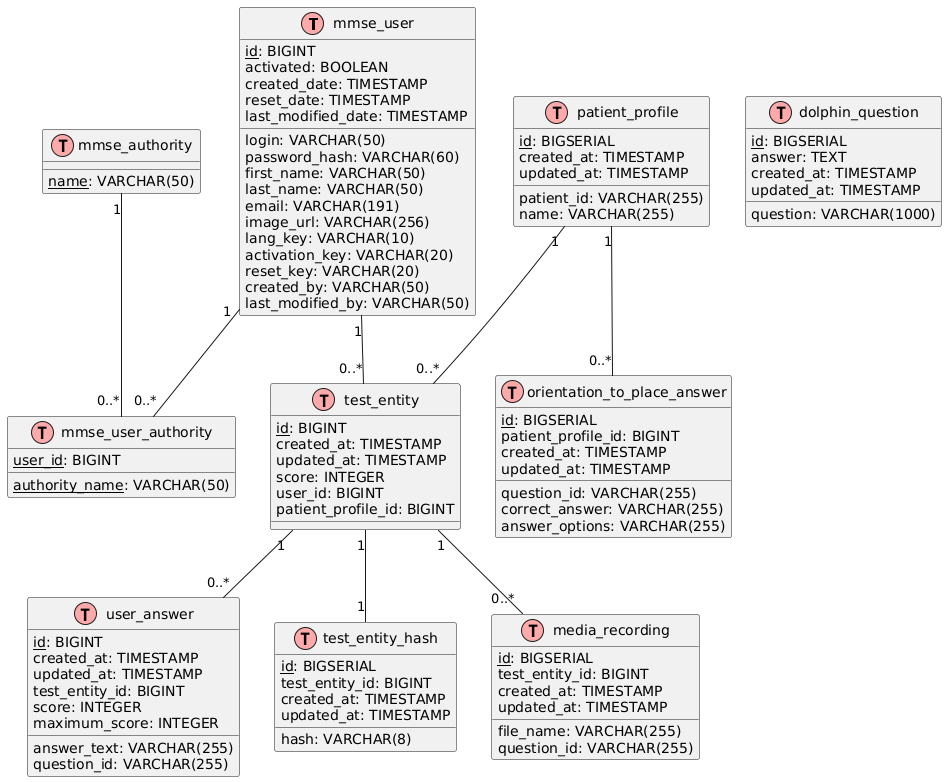
\includegraphics[width=1\textwidth]{er_diagram.png}
\caption{ER Diagram of the AI-Powered Web-based MMSE Application}
\label{fig:er_diagram}
\end{center}
\end{figure}

In our design, several key architectural decisions have been made:
\begin{itemize}
    \item Use of a \textbf{BaseEntity} class: All entities inherit from this class, which provides common fields like \texttt{id}, \texttt{createdAt}, and \texttt{updatedAt}. This approach promotes code reuse and ensures consistent auditing between entities.
    \item Implementation of \textbf{enum types}: Enums like \texttt{QuestionId} ensure type safety and improve the readability of the code.
\end{itemize}

The service layer acts as an intermediary between the domain model and the rest of the application, implementing core business logic and managing data operations. Key service classes include:
\begin{itemize}
    \item \textbf{TestEntityService}: Manages CRUD operations for cognitive tests.
    \item \textbf{QuizService}: Handles the flow of questions and answers during a test session.
    \item \textbf{PatientProfileService}: Manages patient data and history.
\end{itemize}

These services encapsulate complex business logic, such as test-scoring algorithms and patient data analysis. For example, the \texttt{QuizService} class contains methods to retrieve the next question based on previous answers, implementing adaptive testing strategies.

\begin{lstlisting}[language=Java, caption=QuizService adaptive testing method]
public QuestionDTO getNextQuestion(Long testEntityId) {
    Optional<UserAnswer> latestAnswer = userAnswerService.getLatestByTestEntityId(testEntityId);
    if (latestAnswer.isEmpty()) {
        return quizService.getQuestion(QuestionId.QUESTION_1, testEntityId);
    }
    Optional<QuestionId> nextQuestionId = getNextQuestionId(latestAnswer.get().getQuestionId());
    if (nextQuestionId.isEmpty()) {
        // End of test logic
        return null;
    }
    return quizService.getQuestion(nextQuestionId.get(), testEntityId);
}
\end{lstlisting}

To ensure data integrity and improve performance, several strategies are used:
\begin{itemize}
    \item \textbf{Transactional methods}: Critical operations, such as saving test results, are wrapped in transactions to ensure atomicity.
    \item \textbf{Caching}: Redis is used to cache frequently accessed data, such as patient profiles and test configurations, reducing database load, and improving response times.
\end{itemize}

\subsubsection{Question Interface}
The \texttt{Question} interface defines the common structure for different questions in the MMSE application. It includes methods for retrieving the question text, image, question ID, and type. The interface provides default implementations for several methods, allowing subclasses to override these methods as needed. Key methods include:
\begin{itemize}
    \item \texttt{getImage()}: Returns an image associated with the question.
    \item \texttt{getAnswerOptions(Long testEntityId)}: Provides specific answer options for the question.
    \item \texttt{convertImageToBase64(String imagePath)}: Converts an image to a Base64 string, useful for embedding images directly in the application.
    \item \texttt{getMaximumScore()}: Specifies the maximum score for a question.
    \item \texttt{isOrientationToPlace()}: Indicates if the question assesses orientation to place.
    \item \texttt{getLLMPrompt(String input)}: Generates prompts for large language models (LLMs) based on user input.
    \item \texttt{getInstructions()}: Provides specific instructions for the question.
\end{itemize}

The \texttt{getScore(UserAnswer userAnswer)} method is abstract and must be implemented by subclasses, defining how the user’s answer should be evaluated and scored. For information about the complete implementation, please refer to the project repository in the Appendix \ref{appendix:repository}.

\subsubsection{REST API and AI Integration}
The API includes endpoints for managing test sessions, questions and answers, and files associated with specific test sessions. These endpoints enable seamless interaction between the client and server, adhering to RESTful principles and ensuring secure and consistent communication across the system.

Security is a paramount concern in the backend architecture. Various mechanisms are used to protect sensitive data and the system's integrity.
\begin{itemize}
    \item \textbf{Authentication Mechanism (JWT)}: The backend employs JSON Web Tokens (JWT) for authentication \cite{Jones2015}. JWTs are issued to authenticated users and must be included in the Authorization header of subsequent requests.
    \item \textbf{Authorization and Role-Based Access Control}: Role-based access control (RBAC) restricts access to specific endpoints and operations based on the user's role. This mechanism helps enforce the principle of least privilege.
\end{itemize}

The backend integrates with several AI services to enhance the application's cognitive assessment capabilities.
\begin{itemize}
    \item \textbf{OpenAI Service Integration}: The \texttt{OpenAiService} integrates with the ChatGPT models for advanced question evaluation. It handles tasks such as natural language understanding and response generation.
    \item \textbf{Ollama Integration}: The \texttt{DolphinService} uses the Llama 3.1:70B model for specific tasks, such as evaluating orientation questions.
    \item \textbf{Transcription Service}: The transcription service integrates with external APIs to convert audio inputs into text. It processes voice responses, ensuring accurate transcription and handling errors through fallback mechanisms.
    \item \textbf{Prediction and Similarity Services}: These services implement grammar checking and similarity assessment algorithms. They evaluate responses to specific questions, determining thresholds for answer acceptance.
\end{itemize}

The AI-enhanced web-based MMSE application's backend integrates strong domain modeling, effective service layer logic, secure REST API endpoints, and advanced security protocols to build a robust and adaptable system. This design guarantees the application can meet the complex demands of cognitive assessments while upholding superior performance, security, and reliability standards.

Using advanced AI services and adhering to best practices in software design, the backend supports the application's goal of providing comprehensive and accurate cognitive assessments in a digital healthcare setting. The modular and scalable nature of the backend architecture positions the system to evolve alongside advances in AI and cognitive science, ensuring its continued relevance and effectiveness.

A comprehensive fallback mechanism has been implemented to ensure robustness and accuracy in evaluating the responses to the MMSE questions. This mechanism integrates various methods to determine the correctness of an answer, providing multiple layers of validation.

The primary mechanism uses several methods to evaluate the correctness of an answer:
\begin{enumerate}
    \item \textbf{Direct Matching}:
    The first check involves comparing the answer against a predefined list of incorrect answers. If the answer matches any entry in this list, a score of 0 is assigned.

{\footnotesize
\begin{verbatim}
if (INCORRECT_ANSWERS.contains(answerText)) {
    log.debug("Answer '{}' is in the list of incorrect answers.", answerText);
    return 0;
}
\end{verbatim}
}

    \item \textbf{Service-based Matching}:
    The code then checks if the answer is a synonym or similar to accepted answers using the \texttt{synonymService} and \texttt{similarityService}.

{\footnotesize
\begin{verbatim}
if (isSynonym(answerText)) {
    log.debug("Answer '{}' is a synonym to one of the accepted answers.", answerText);
    return 1;
}

if (isSimilar(answerText)) {
    log.debug("Answer '{}' is similar to one of the accepted answers.", answerText);
    return 1;
}

if (isDolphinSimilar(answerText)) {
    log.debug("Answer '{}' is similar to one of the accepted answers.", answerText);
    return 1;
}
\end{verbatim}
}

    \item \textbf{Evaluating OpenAI Response}:
    If the previous methods do not provide a definitive answer, the OpenAI service is queried with the answer. The OpenAI response is evaluated to determine the correctness of the answer.

{\small
\begin{verbatim}
Optional<String> openAiResponse = checkWithOpenAiService(answerText);
return evaluateOpenAiResponse(answerText, openAiResponse);
\end{verbatim}
}

    \item \textbf{Fallback Mechanism}:
    If all the above methods fail to provide a definitive answer, any unhandled scenarios are logged and may be re-evaluated through additional logic. This ensures that the system can handle various response variations and maintain reliability.
\end{enumerate}

This fallback mechanism ensures that the system can accurately and reliably evaluate responses, even in complex or unexpected scenarios. Integrates multiple layers of validation to provide a robust solution for cognitive assessment.

\subsection{Testing Practices}
The MMSE application employs comprehensive testing practices to ensure reliability and accuracy in cognitive assessments:
\begin{enumerate}
\item \textbf{Unit Testing:} Individual components, particularly those related to question handling and scoring, are tested in isolation to verify their functionality under various conditions;
\item \textbf{Integration Testing:} Tests are conducted to ensure smooth interaction between different components of the system, including question creation, retrieval, and response processing;
\item \textbf{Custom Testing Annotations:} A custom \texttt{@IntegrationTest} annotation is used to set up consistent testing environments, including necessary services like Redis;
\item \textbf{Continuous Integration:} An automated pipeline for code integration and testing is implemented, utilizing tools like GitHub Actions to ensure code stability, facilitate quick issue resolution, and improve overall application reliability.
\end{enumerate}
These practices contribute to the robustness of the AI-powered MMSE system, ensuring its effectiveness in cognitive assessment applications. The focus on thorough testing supports the reliability of the results presented in this thesis.

\subsection{Frontend Implementation}
The AI-powered MMSE application frontend is designed to provide a user-friendly interface for healthcare providers and patients. Developed using Vue.js and TypeScript, the frontend ensures a responsive and intuitive experience, facilitating seamless interaction with the underlying AI-powered cognitive assessment tools.

\subsubsection{Component Structure Overview}
The Vue.js application is organized into several key components, each responsible for different aspects of the cognitive assessment process. The primary components include those that manage MMSE-related entities, shared utilities, and the application's routing.

\subsubsection{Interaction with Backend Logic}
The frontend components are primarily responsible for rendering the MMSE test questions, capturing user responses, and communicating with the backend to process these responses. This interaction is crucial for automating the cognitive assessment, allowing for real-time data processing and analysis by the AI-driven backend services.

\subsubsection{User Experience and Interface Design}
The frontend's design focuses on simplicity and usability, ensuring that healthcare providers and patients can easily navigate the application. The use of modern web technologies like Vue.js contributes to a fluid user experience, while the integration with AI services ensures that the cognitive assessments are both accurate and efficient.

\subsection{Data Management}
Effective data management and storage are crucial for the performance and reliability of the AI-enhanced Web-based MMSE application. The system employs a combination of PostgreSQL for persistent storage, Redis for caching frequently accessed data, and MinIO for managing media files. This section details the application's implementation and strategies for data management and storage.

\textbf{Caching Strategy}
To optimize performance and reduce database load, the MMSE application employs Redis for caching frequently accessed data. This strategy is particularly beneficial for:
\begin{itemize}
\item user session data, enabling quick retrieval of user states;
\item test results and configuration data, reducing repetitive database queries.
\end{itemize}
The caching system implements Time-To-Live (TTL) policies and cache invalidation methods to ensure data consistency. TTL values are assigned based on data volatility, while manual and event-driven invalidation mechanisms maintain cache accuracy.
This approach significantly improves response times for frequently used queries, enhancing the overall user experience and system efficiency.

\textbf{MinIO for Media Storage}

MinIO is integrated into the MMSE application to manage media files, including the storage, retrieval, and deletion of these files. The StorageService class handles all file operations, ensuring that media files are managed efficiently and securely.
Key features of the StorageService include:
\begin{itemize}
\item secure file upload functionality, generating unique identifiers for each file;
\item efficient file retrieval mechanism;
\item integration with MinIO, a high-performance object storage system;
\item error handling for upload and download operations.
\end{itemize}
This implementation ensures that the MMSE application can effectively manage and access media files associated with cognitive assessments, while maintaining data integrity and security.

\textbf{Security Measures for Media Files}
To protect the integrity and confidentiality of media files, the application implements several security measures:
\begin{itemize}
\item role-based access control (RBAC) to restrict file access to authorized users only;
\item encryption of data in transit using HTTPS protocol;
\item secure storage of media files using MinIO, with potential for server-side encryption at rest.
\end{itemize}
These measures are crucial in healthcare applications to protect patient data and comply with data privacy regulations. While the current implementation provides a foundation for secure media file handling, further configuration may be necessary to fully meet the highest data security and privacy standards in a production environment (Krutz 2017).